\documentclass[12pt]{article}
\usepackage[letterpaper,margin=1in]{geometry}
\usepackage{newtxtext,newtxmath}
\usepackage{amsmath}
\usepackage{bm}
\usepackage{enumitem}
\usepackage{pdfpages}
\usepackage{fancyhdr}

\bmdefine{\ii}{i}
\bmdefine{\jj}{j}
\bmdefine{\kk}{k}

\setlength{\parindent}{0pt}
\pagestyle{fancy}
\fancyhf{}
\fancyfoot[R]{\thepage}
\renewcommand{\headrulewidth}{0pt}
\renewcommand{\footrulewidth}{0pt}

\begin{document}

% Question 1 is reproduced exactly from the source PDF. It is a matching
% problem and therefore does not receive an answer box.
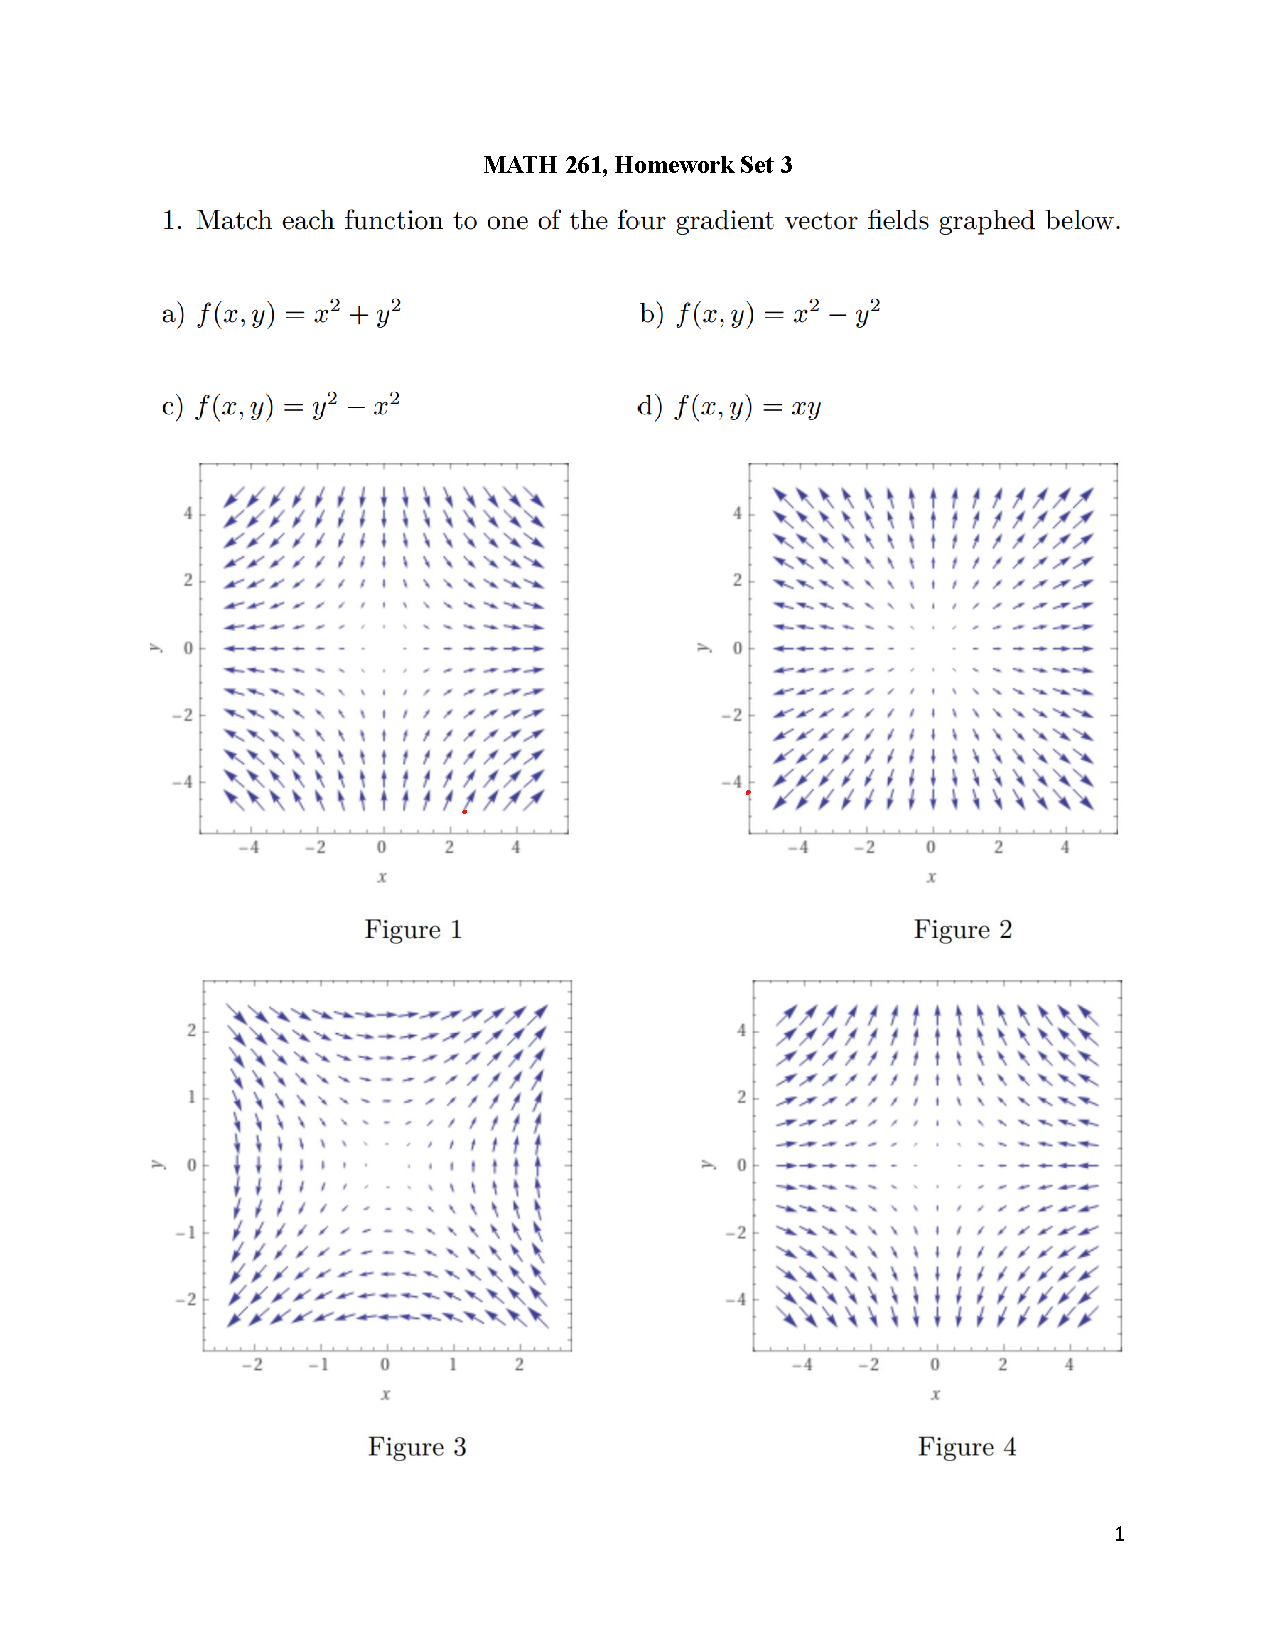
\includepdf[pages=1,pagecommand={\thispagestyle{empty}}]{HW3_Fall2025.pdf}

\setcounter{page}{2}
\begin{enumerate}[label=\arabic*.,start=2,leftmargin=*,itemsep=0pt]

\item Let $f(x,y)=x^3y+y^2x^2+x^4$. Compute a formula for the two dimensional
gradient vector, $\nabla f(x,y)$.

\vfill
\begin{flushright}
\framebox(250,50){}
\end{flushright}

\item Let $f(x,y,z)=x^2\sin(1+y^2)+z^3$. Compute a formula for the three
dimensional gradient vector, $\nabla f(x,y,z)$.

\vfill
\begin{flushright}
\framebox(250,50){}
\end{flushright}

\newpage

\item Let $f(x,y)=y^2\sin(xy)$. In which direction is this function increasing
the fastest at the point $(0,2)$? In which direction is it decreasing the
fastest?

\vfill
\begin{flushright}
\framebox(250,50){}
\end{flushright}

\item Let $f(x,y)=ye^x+x^2$. In which direction is this function increasing
the fastest at the point $(0,0)$? In which direction is it decreasing the
fastest?

\vfill
\begin{flushright}
\framebox(250,50){}
\end{flushright}

\newpage

\item Let $f(x,y)=y^4-4x^2+5$. In which direction is this function increasing
the fastest at the point $(1,1)$? In which direction is it decreasing the
fastest?

\vfill
\begin{flushright}
\framebox(250,50){}
\end{flushright}

\item Let $f(x,y,z)=x^2y^2+z^4$. In which direction is this function
increasing the fastest at the point $(1,1,-1)$? In which direction is it
decreasing the fastest?

\vfill
\begin{flushright}
\framebox(250,50){}
\end{flushright}

\newpage

\item Let $f(x,y,z)=xy^2z^4$. In which direction is this function increasing
the fastest at the point $(0,-2,1)$? In which direction is it decreasing the
fastest?

\vfill
\begin{flushright}
\framebox(250,50){}
\end{flushright}

\item Compute $D_{\vec{u}}f(x,y)$, where $\vec{u}$ points in the direction of
$(1,1)$ and $f(x,y)=xy^2$, at the point $(2,2)$.

\vfill
\begin{flushright}
\framebox(250,50){}
\end{flushright}

\newpage

\item Compute $D_{\vec{u}}f(x,y)$, where $\vec{u}$ points in the direction of
$(0,-1)$ and $f(x,y)=xy^2$, at the point $(2,2)$.

\vfill
\begin{flushright}
\framebox(250,50){}
\end{flushright}

\item Suppose that $D_{\vec{u}}f(x,y,z)$ is large and positive at $(0,0,0)$,
for a unit vector $\vec{u}$. What does this tell about $f(x,y,z)$? Suppose that
$D_{\vec{u}}f(x,y,z)$ was zero at the origin instead---what would that tell
you?

\vfill
\begin{flushright}
\framebox(250,50){}
\end{flushright}

\newpage

\item Suppose $\nabla f=(1,2,-1)$ at $(0,0,0)$ for a function $f(x,y,z)$.
What is $D_{\vec{u}}f(0,0,0)$ if $\vec{u}=(0,1,3)$? Is the function increasing
or decreasing?

\vfill
\begin{flushright}
\framebox(250,50){}
\end{flushright}

\item Compute the function $D_{\vec{u}}f(x,y,z)$, where
$f(x,y,z)=yze^x+1$ and $\vec{u}$ points in the direction of
$1\ii+0\jj+1\kk$.

\vfill
\begin{flushright}
\framebox(250,50){}
\end{flushright}

\newpage

\item Compute the function $D_{\vec{u}}f(x,y,z)$, where
$f(x,y,z)=xy^2+ye^z$ and $\vec{u}$ points in the direction of
$1\ii+0\jj+2\kk$.

\vfill
\begin{flushright}
\framebox(250,50){}
\end{flushright}

\item Compute the function $D_{\vec{u}}f(x,y,z)$, where
$f(x,y,z)=\dfrac{y}{x^2+1}+z^8$ and $\vec{u}$ points in the direction of
$1\ii-1\jj+0\kk$.

\vfill
\begin{flushright}
\framebox(250,50){}
\end{flushright}

\newpage

\item Explain, geometrically, why $f_x$ and $f_y$ must both be zero at a local
maximum or local minimum of a smooth function $f(x,y)$.

\vfill
\begin{flushright}
\framebox(250,50){}
\end{flushright}

\item Show that $(0,0)$ is a critical point of the function
$f(x,y)=x^2+3y^2+x^3y^3$. Use the second partial derivative test to classify
this as a local maximum, local minimum, or neither.

\vfill
\begin{flushright}
\framebox(250,50){}
\end{flushright}

\newpage

\item Show that $(1,1)$ is a critical point of the function
$f(x,y)=x^2+y^2-2x-2y$. Use the second partial derivative test to classify this
as a local maximum, local minimum, or a saddle point.

\vfill
\begin{flushright}
\framebox(250,50){}
\end{flushright}

\item Show that $(1,3)$ is a critical point of the function
$f(x,y)=6y+2x-x^2-y^2+10$. Use the second partial derivative test to classify
this as a local maximum, local minimum, or a saddle point.

\vfill
\begin{flushright}
\framebox(250,50){}
\end{flushright}

\newpage

\item Show that $(1,1)$ is a critical point of the function
$f(x,y)=x^2-2x-y^2+2y+18$. Use the second partial derivative test to classify
this as a local maximum, local minimum, or a saddle point.

\vfill
\begin{flushright}
\framebox(250,50){}
\end{flushright}

\item Show that $(0,0)$ is a critical point of the function
$f(x,y)=x^3y+xy$. Use the second partial derivative test to classify this as a
local maximum, local minimum, or a saddle point.

\vfill
\begin{flushright}
\framebox(250,50){}
\end{flushright}

\newpage

\item Find a vector normal to the surface $x^2+y^2-z^2=6$ at the point
$(3,1,2)$.

\vfill
\begin{flushright}
\framebox(250,50){}
\end{flushright}

\item Find a vector normal to the surface $3z^3+x^2y-y^2x=1$ at the point
$(1,-1,1)$.

\vfill
\begin{flushright}
\framebox(250,50){}
\end{flushright}

\newpage

\item Find an equation of the tangent plane to the surface
$x^2+3y^2+4z^2=20$ at the point $(2,2,1)$.

\vfill
\begin{flushright}
\framebox(250,50){}
\end{flushright}

\item Find an equation of the tangent plane to the surface
$xz+2x^2y+y^2z^3=11$ at the point $(2,1,1)$.

\vfill
\begin{flushright}
\framebox(250,50){}
\end{flushright}

\end{enumerate}

\end{document}
